%%%% ijcai11.tex

\typeout{IJCAI-11 Instructions for Authors}

% These are the instructions for authors for IJCAI-11.
% They are the same as the ones for IJCAI-07 with superficical wording
%   changes only.

\documentclass{article}
% The file ijcai11.sty is the style file for IJCAI-11 (same as ijcai07.sty).
\usepackage{ijcai11}
\usepackage{mathtools}
\usepackage[utf8]{inputenc}
\usepackage{amsmath}
\usepackage{slashbox}

% For importing images.
\usepackage{graphicx}

% The language we want and appropriate hyphenation.
\usepackage[dutch]{babel}

% Hyphenation rules.
\hyphenation{biopotentiaal-schommelingen}

% Use the postscript times font!
\usepackage{times}

% the following package is optional:
%\usepackage{latexsym} 


\title{Kijkrichtingen detecteren door middel van elektromyografie}
\author{Kevin Boets \\ Katholieke Universiteit Leuven\\ Departement Computerwetenschappen \\ kevin.boets@student.kuleuven.be
\And
Gertjan Franken \\ Katholieke Universiteit Leuven\\ Departement Computerwetenschappen \\ gertjan.franken@student.kuleuven.be}

\begin{document}

\maketitle

\begin{abstract}
In de zoektocht naar natuurlijke user interfaces gebeurt er onderzoek naar besturing door middel van de ogen. In deze paper wordt gebruik gemaakt van EMG (Elektromyografie) signalen om eenvoudige oogbewegingen te detecteren. Hiervoor onderzoeken we twee verschillende methodes: thresholds en patronen. Beide methodes worden dan ook grondig besproken en vergeleken doorheen de tekst.
\end{abstract}

\section{Introductie}

Reeds verschillende manieren om oogbewegingen te detecteren zijn bedacht. Zo kan men al door middel van camera's de ogen volgen. Hierbij gaat men op zoek naar de positie van de iris om de stand van het oog te achterhalen. Deze technieken zijn al ver ontwikkeld, maar bieden nog geen oplossing voor alle problemen. Daarom onderzoeken wij een andere manier. We maken gebruik van sensoren die rond de ogen zijn aangebracht, om elektromyografie (EMG) signalen te meten. Aan de hand van deze signalen proberen we te achterhalen in welke richting de gebruiker kijkt. Als invoer krijgen we twee elektrooculogrammen die respectievelijk de kijkrichtingen links-rechts en boven-onder voorstellen. Figuur~\ref{fig:originaldata} geeft een mooi voorbeeld weer van het elektrooculogram betreffende de kijkrichtingen links en rechts. Hierbij stellen de dalen de kijkrichting links voor en stellen de bergen de kijkrichting rechts voor.

\section{Preprocessing}

Het signaal dat we krijgen doorgestuurd, afkomstig van de sensoren, is zeer ruw. Om hier kijkrichtingen uit af te kunnen leiden, gaan we de data eerst beter leesbaar maken. Dit is de preprocessing-stap. Deze stap voeren we uit op elke dataset,  alvorens we deze gaan analyseren. Beschouw de data in figuur~\ref{fig:originaldata} als de originele data.

\begin{figure}[h]
\centering
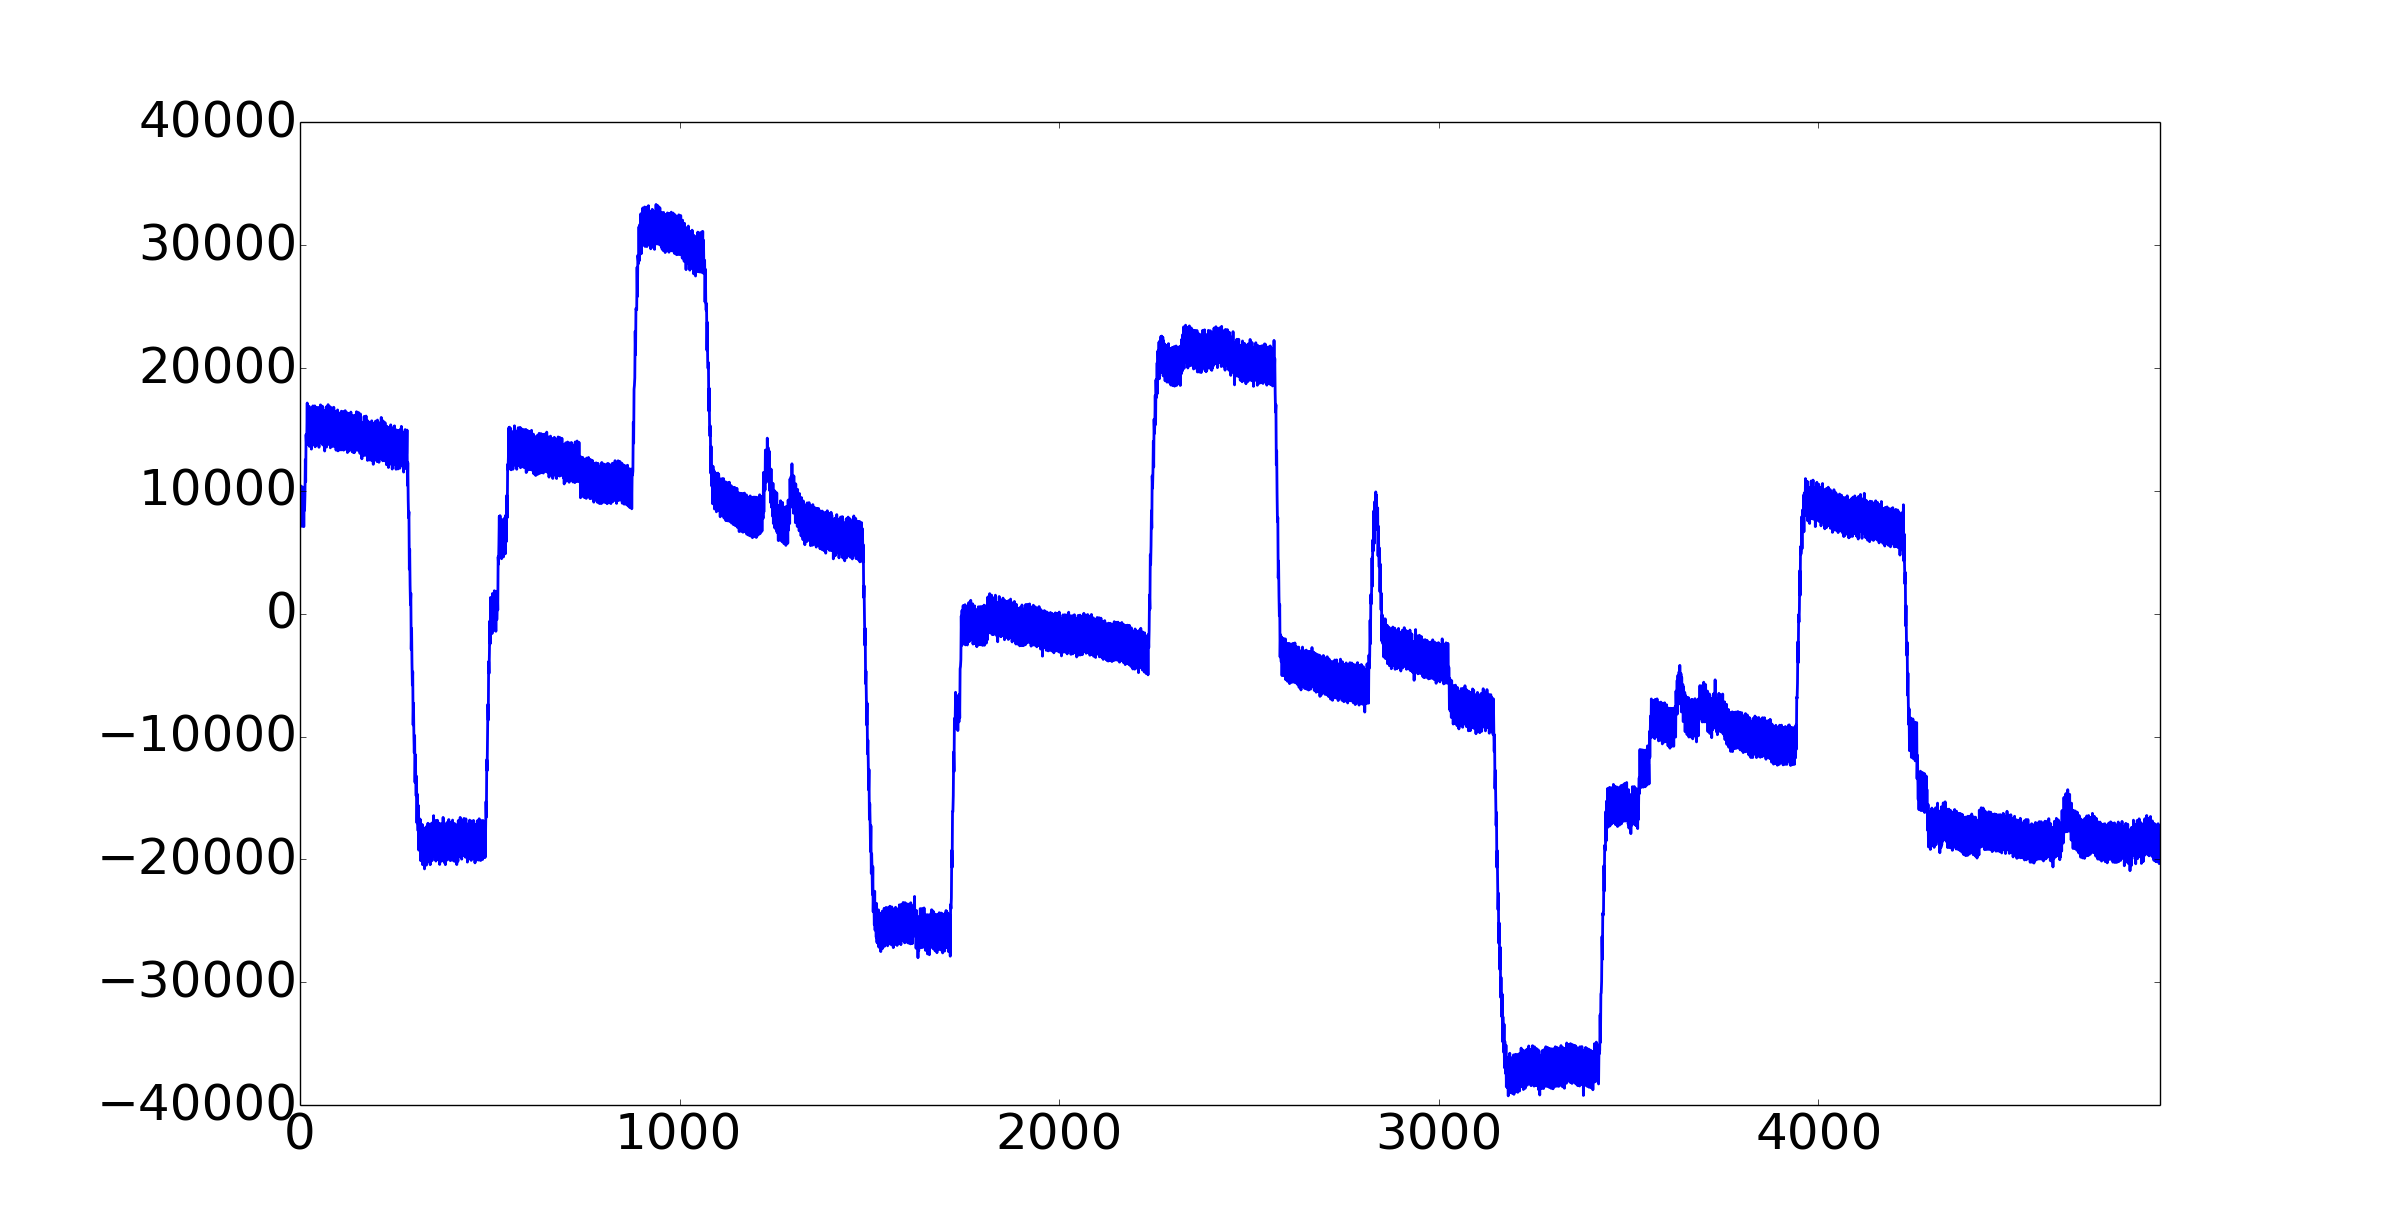
\includegraphics[width=\linewidth]{images/original_data}
\caption{Originele data rechtstreeks afkomstige van de hardware. De grootheid op de x-as is tijd en op de y-as is dit het voltage.}
\label{fig:originaldata}
\end{figure}

Als eerste gaan we de ruis en knipperingen zo goed mogelijk proberen te verminderen. Dit gebeurt door middel van een low-pass filter. Deze filter verzacht het signaal door de hoogfrequentie te verminderen. Dit gebeurt in vergelijking~\ref{eq:ruisfiltering}, waarbij $s$ het originele signaal is. Hierbij geven we ook een andere variabele, de cutoff frequentie $cf_1$, mee zodat alle frequenties hoger dan deze variabele worden afgezwakt. Wij geven $cf_1$ de waarde [TODO].

\begin{equation}
\label{eq:ruisfiltering}
s' = lowpass(s, cf_1)
\end{equation}

Daarna focussen we ons op de biopotentiaalschommelingen. Deze schommelingen kunnen we niet op voorhand voorspellen en verschillen van persoon tot persoon. Als we deze schommelingen kunnen verminderen, kunnen we meer steunen op absolute waarden van het signaal. In dit tweede deel van de preprocessing-stap gebruiken we opnieuw een low-pass filter. Deze keer gebruiken we een lage cutoff frequentie $cf_2$ met de waarde [TODO]. Na deze filtering van de data, blijven enkel de signalen met een lage frequentie over. Het resultaat is de benadering van de biopotentiaal van de gebruiker die doorheen de tijd fluctueert. We kunnen nu de biopotentiaalschommelingen uit onze originele data verminderen door de gevonden benadering hiervan af te trekken, zoals in vergelijking~\ref{eq:aftrekkingbiopotentiaal}. De schommelingen verdwijnen niet volledig, maar worden wel sterk verminderd. Figuur~\ref{fig:filtereddata} stelt het resultaat van de besproken filtereringen voor.

\begin{equation}
\label{eq:aftrekkingbiopotentiaal}
s'' = s' - lowpass(s', cf_2)
\end{equation}

Bij veelvuldige herhaling van dezelfde kijkrichting, wordt een probleem in verband met deze methode zichtbaar. Als er veel en opeenvolgend naar éénzelfde richting gekeken wordt, zullen de waarden in de data algemeen lager of hoger zijn. De gefilterde data zal hierdoor ook algemeen lager of hoger liggen. Dit is een probleem aangezien het de benadering van de biopotentiaal moet voorstellen. Doordat de gevonden benadering foutief is, zullen ook alle volgende bewerkingen een incorrecte uitkomst hebben. Wanneer we dus deze benadering aftrekken van de oorspronkelijke data, zal de data ongewenst verschuiven volgens de y-as. Hierdoor zal het werken met absolute waarden slechte resultaten opleveren. Omdat de gebruiker zelf kiest welke reeks van kijkrichtingen hij uitvoert, moeten we hier een oplossing voor vinden voor de gevallen waarbij we deze absolute waarden nodig hebben.

\begin{figure}[h]
\centering
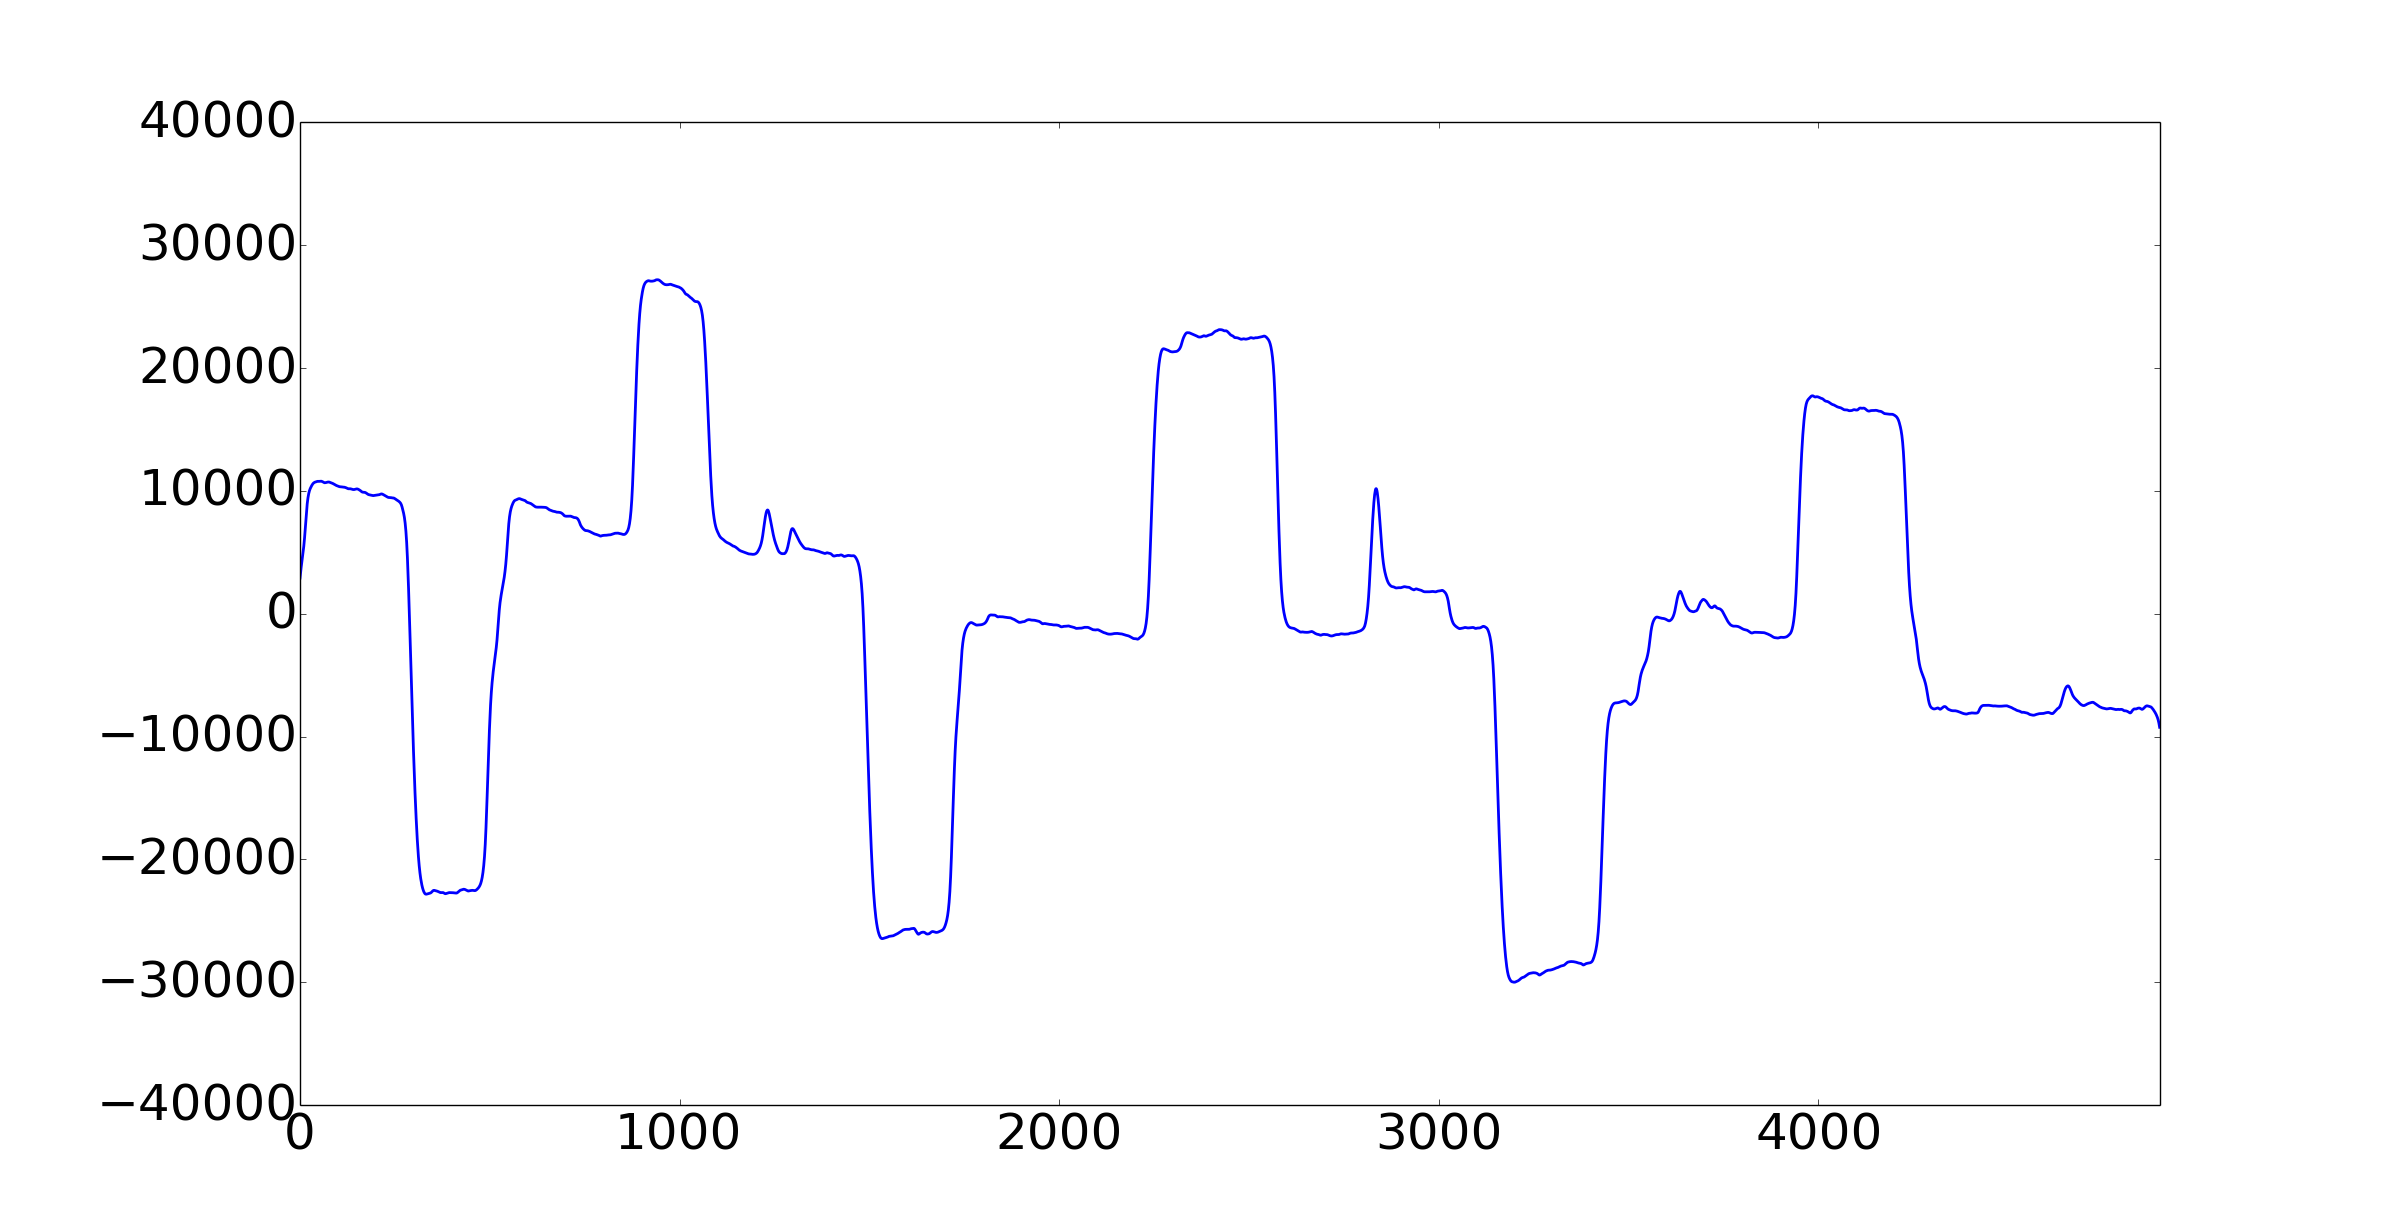
\includegraphics[width=\linewidth]{images/filtered_data}
\caption{Het resultaat van de twee filteringen op de originele data. De ruis is sterk verminderd en de sterkte van de knipperingen is afgenomen. De biopotentiaalschommeling is niet helemaal weg, maar wel voldoende verminderd.}
\label{fig:filtereddata}
\end{figure}

Na toepassing van de vorige filteringen, discretiseren we de data. Deze stap is eerder optioneel en wordt enkel in de methode met patronen gebruikt. Het grote voordeel van deze stap is dat we minder berekeningen zullen moeten doen, wat de uitvoeringstijd van het programma ten goede komt. Hiervoor gebruiken we de SAX-discretisatie (Symbolic Aggregate approXimation) \cite{sax}. Eerst wordt de data genormaliseerd. We definiëren op voorhand hoeveel waarden een letter voor moet stellen. Dit is de constante $w$. De data die we willen discretiseren, verdelen we op in partities van lengte $w$. Elke partitie zal een bepaalde letter krijgen, afhankelijk van zijn gemiddelde. Het aantal verschillende letters dat we gebruiken, hangt af van de alfabetgrootte $a$. Volgens de normale verdeling wordt nu elke partitie aan een letter gekoppeld. Zie figuur~\ref{fig:discretization} voor de visuele werking. Eigenlijk stelt elke letter nu een reeks van waarden voor. Om SAX-woorden voor te kunnen stellen in grafieken, geven we elke letter ook een waarde. Dit is het gemiddelde van de intervalgrenzen die de letter op zicht neemt.

\begin{figure}[h]
\centering
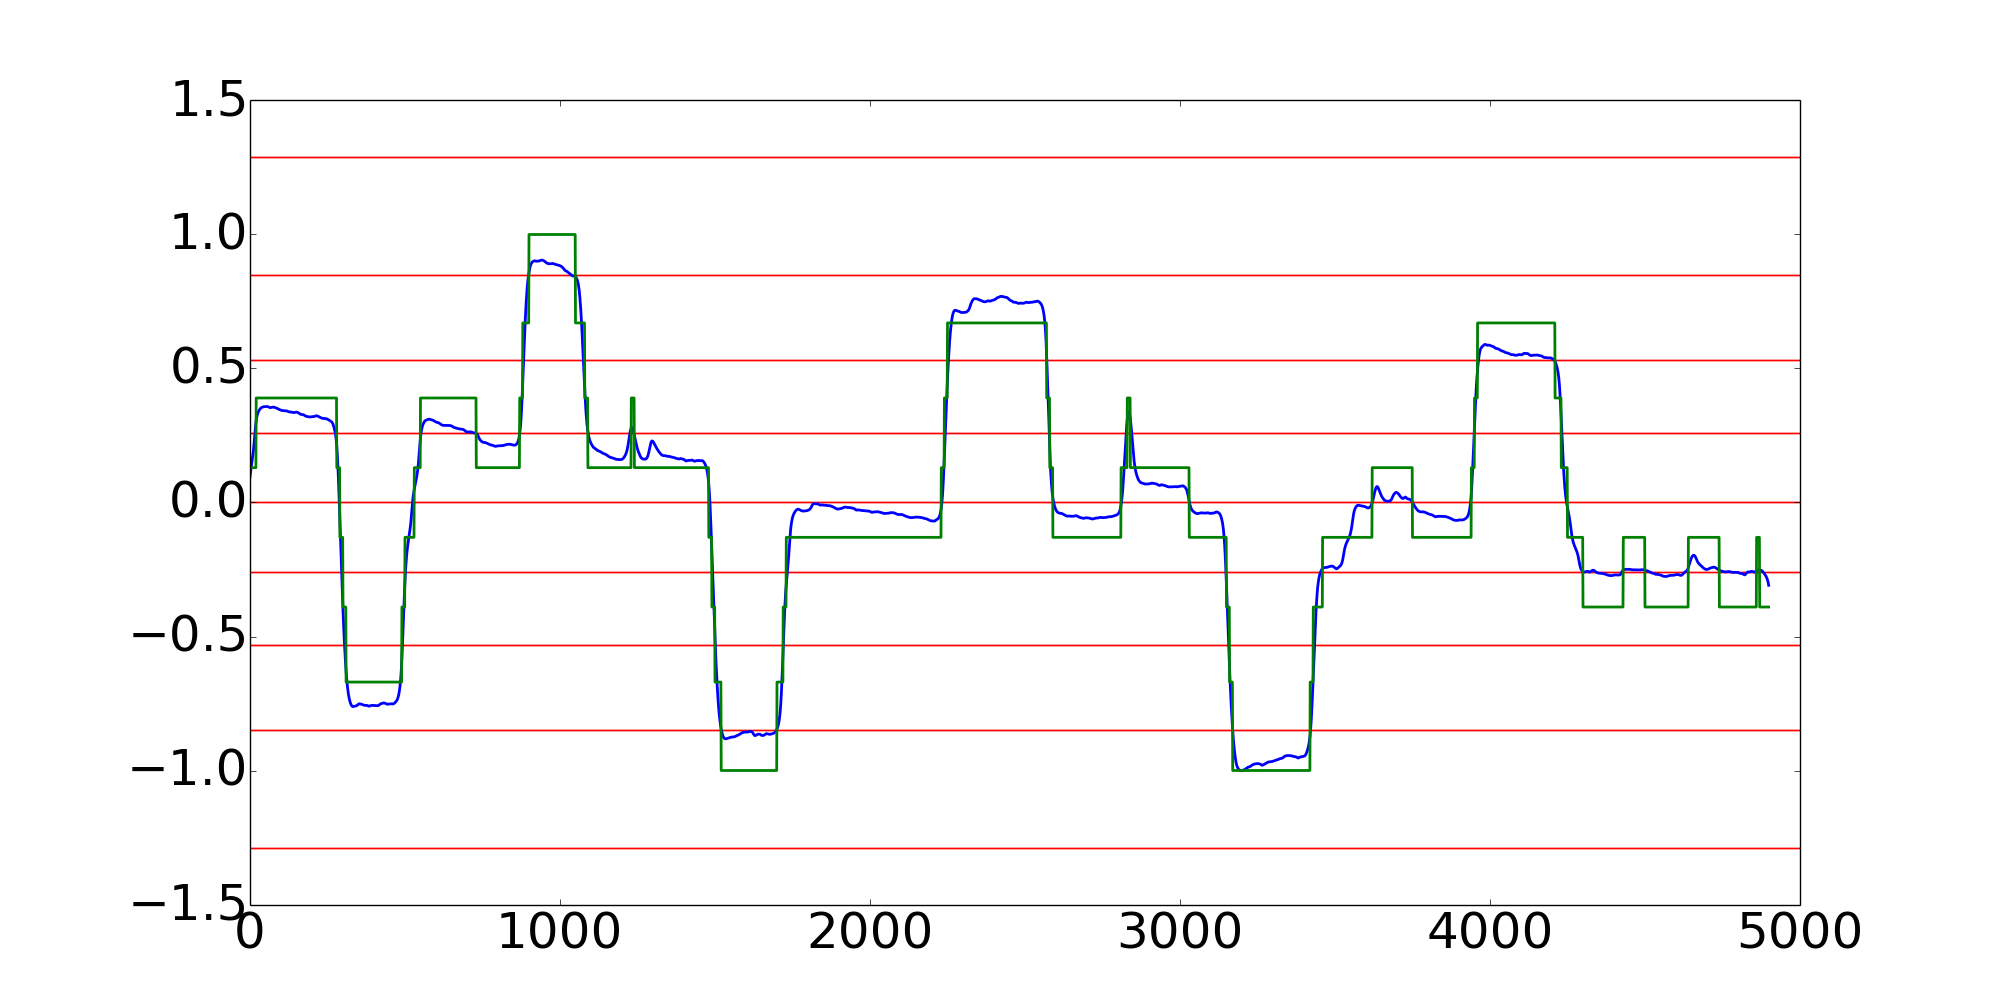
\includegraphics[width=\linewidth]{images/sax_normaal_verdeling}
\caption{De groene lijn stelt de discretisatie voor van de gefilterde data die in het blauw staat. De rode horizontale lijnen geven de distributie weer van de SAX-letters. Deze distributie is volgens de normale verdeling met gemiddelde 0 en standaarddeviatie 1.}
\label{fig:discretization}
\end{figure}

\section{Gebruikte methoden}

In ons onderzoek hebben we gebruik gemaakt van twee verschillende methoden om kijkrichtingen te herkennen. Deze methoden steunen respectievelijk op thresholds en patronen. Beide methoden beginnen met een calibratie-fase, gevolgd door een herkennings-fase. In de calibratie-fase laten we de gebruiker naar een aantal richtingen kijken, waarna we deze data analyseren. De gevonden informatie koppelen we aan de juiste kijkrichting. In de herkennings-fase wordt deze informatie gebruikt om in de nieuwe data kijkrichtingen te detecteren.

\subsection{Thresholds}

De eenvoudigste methode is de methode gebruikmakend van thresholds. Het steunt vooral op de absolute waarden van de data. Het basis idee van deze methode is als volgt. Er wordt een bovengrens gedefinieerd voor elke kijkrichting in de calibratie-fase. Als deze overschreden wordt in de herkennings-fase, gaan we er van uit dat er in de overeenkomstige kijkrichting gekeken wordt.

In de calibratie-fase wordt aan de gebruiker gevraagd om een bepaalde sequentie van kijkrichtingen uit te voeren. Vervolgens voeren we de preprocessing-stap uit in verband met de ruis, knipperingen en biopotentiaal. Hier maken we geen gebruik van de SAX-discretisatie omdat deze methode al efficiënt genoeg is. De preprocessed dataset gebruiken we dan om goede bovengrenzen te vinden. Figuur~\ref{fig:thresholds} illustreert een voorbeeld van welke bovengrenzen gebruikt kunnen worden op het signaal dat we eerder al hadden besproken.

\begin{figure}[h]
\centering
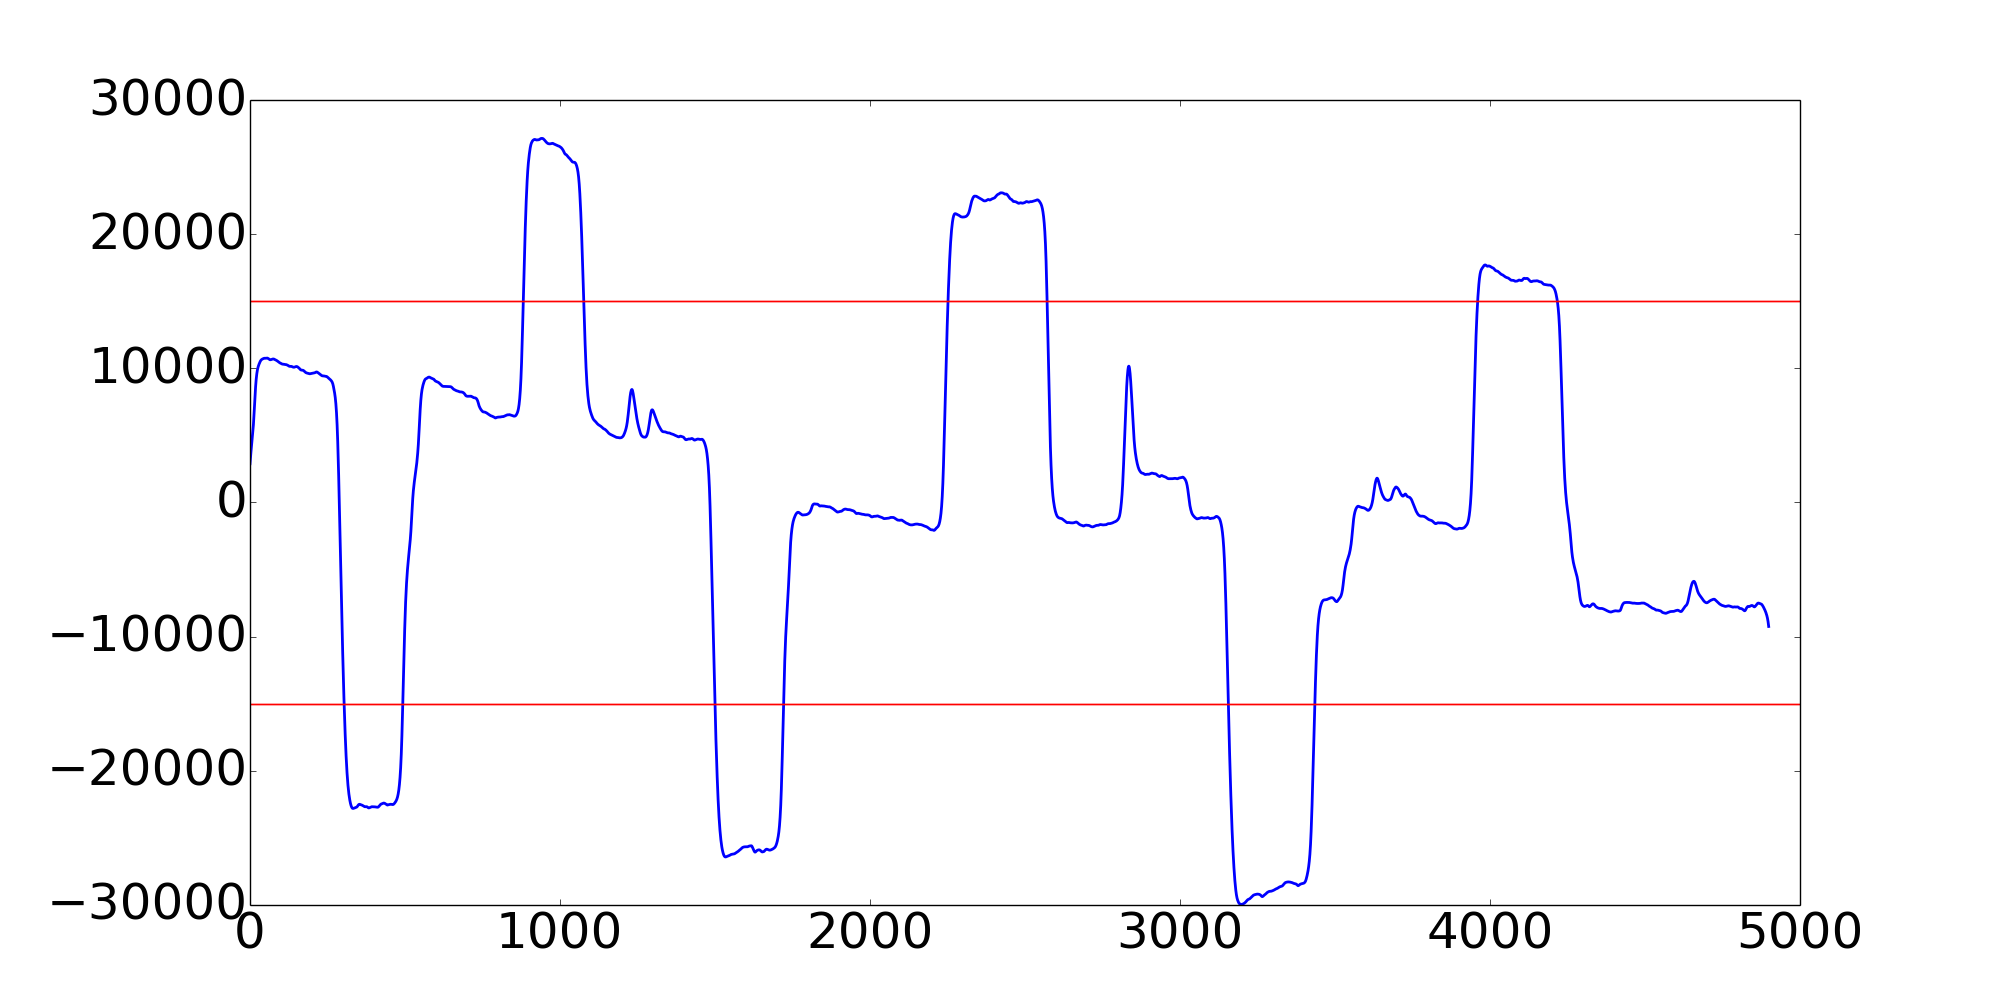
\includegraphics[width=\linewidth]{images/thresholds_voorbeeld}
\caption{In deze afbeelding stellen de rode horizontale lijnen mogelijke bovengrenzen voor.}
 \label{fig:thresholds}
\end{figure}

Eens we de bovengrenzen hebben gevonden, kunnen we deze in de herkennings-fase gebruiken om kijkrichtingen te detecteren. Om deze gevonden bovengrenzen te kunnen gebruiken, zullen we eerst dezelfde preprocessing stappen utivoeren op de nieuwe data. Belangrijk is dat we het signaal ten allen tijde stabiel houden, we werken immers met absolute waarden.

Om kijkrichtingen te detecteren, gaan we de bovengrenzen vergelijken met de waardes uit de data. Wanneer een bovengrens overschreden wordt, toont dit aan dat de gebruiker mogelijk in een van de richtingen aan het kijken is. Dit kunnen we echter niet zomaar aannemen. Een enkele piek, zoals een knippering, zou dan ook ongewild worden herkend als kijkrichting. Om voor meer zekerheid te zorgen, wachten we tot dezelfde grens opeenvolgend meerdere keren overschreden is. Hoeveel keren definiëren we op voorhand. Het aantal dat we kiezen is een afweging tussen detectiekans en zekerheid. Bij een klein aantal is de kans op detectie hoog, maar zijn we minder zeker over de geldigheid van de detectie. Een groot aantal zal anderzijds veel zekerheid verschaffen, waarbij er wel een grotere kans is dat korte kijkrichtingen niet worden gedetecteerd. Hierbij is een goede balans belangrijk.

\subsection{Patronen}

In tegenstelling tot de thresholds-methode, steunt deze methode weinig op absolute waarden en eerder op relatieve waarden. Er wordt naar veel voorkomende patronen gezocht in de calibratie-fase, die dan in de herkennings-fase met de nieuwe data vergeleken worden \cite{motifs}. Deze patronen worden motieven genoemd. In deze methode maken we gebruik van de SAX-discretisatie om de efficiëntie te verhogen.

Ook hier wordt in de calibratie-fase aan de gebruiker gevraagd om in een aantal kijkrichtingen te kijken. Voor elke kijkrichting hebben we nu een aantal datasets van signalen die we met elkaar gaan vergelijken. Voor elke kijkrichting zoeken we de meest succesvolle motieven. Dit zijn de motieven die het meest aantal matches hebben. We zeggen dat twee sequenties met elkaar matchen indien deze voldoende hard op elkaar lijken. Hiervoor moeten specifieke voorwaarden gedefinieerd worden. Dit doen we voor ons programma in de implementatie-sectie.

In de paper \cite{motifs} gebruikt men collision matrices om zo efficiënt mogelijk de motieven te vinden. Hierop hebben we ons gebaseerd en dit wordt dan ook uitgebreid uitgelegd in de implementatie-sectie.

De gevonden motieven, gekoppeld aan de bijhorende kijkrichtingen, worden doorgegeven aan de herkennings-fase. De binnenkomende data wordt verdeeld in sequenties die omgezet worden in SAX-woorden. Pas als er voldoende overeenkomst is tussen een binnengekomen SAX-woord en een SAX-woord van een motief, vergelijken we deze sequenties op preciezer niveau. Als deze sequenties weer goed genoeg op elkaar lijken, vermoeden we dat de kijkrichting gekoppeld aan het herkende motief is uitgevoerd.

\section{Implementatie}

Bij het implementeren van ons programma, hebben we ons gebaseerd op de twee eerder uitgelegde methoden. In deze sectie leggen we uit hoe we de implementatie hebben verwezelijkt. Hierbij geven we ook weer hoe we bepaalde problemen hebben opgelost.

In beide methodes gebruiken we een buffer die de 500 recentste datapunten bijhoudt. Om de 10 datapunten die we ontvangen van de sensoren, wordt deze buffer geupdate. De 10 oudste puntent worden verwijderd en de 10 recentste punten worden vooraan toegevoegd. Elke keer als dit gebeurt, voeren we ook de preprocessing-stap uit op de data in de buffer. Deze buffer wordt ook getoond aan de gebruiker tijdens de uitvoering van het programma. In het begin van het programma wordt ook altijd een buffer fill uitgevoerd. Hierbij laten we de gebruiker voor zich uit kijken tot dat de buffer helemaal gevuld is.

\subsection{Thresholds}

In de calibratie-fase gaan we dus opzoek naar goede bovengrenzen. Nadat de preprocessing-fase is voltooid op de dataset, halen we er de kleinste en grootste waarde uit. Deze twee waarden horen elk bij een andere kijkrichting. Per kijkrichting hebben we ook een constante $\alpha$ waarvoor geldt: $0 < \alpha \leq 1$. We vermenigvuldigen $\alpha$ met het minimum of maximum (afhankelijk van de kijkrichting) en beschouwen de uitkomst als de uiteindelijke bovengrens voor de kijkrichting. Dit wordt aangetoond in figuur~\ref{fig:maxminthresholds}.

In ons programma hebben we $\alpha$ voor beide kijkrichtingen de waarde $0.5$ gegeven, maar deze kan veranderd worden naar behoefte. Zo kunnen we de methode bijvoorbeeld strenger maken door $\alpha$ te verhogen. Het kan ook voorkomen dat het signaal bij de ene kijkrichting sterker uitwijkt dan bij de andere. In dit geval kan de $\alpha$ van deze kijkrichting verminderd worden.

\begin{figure}[h]
\centering
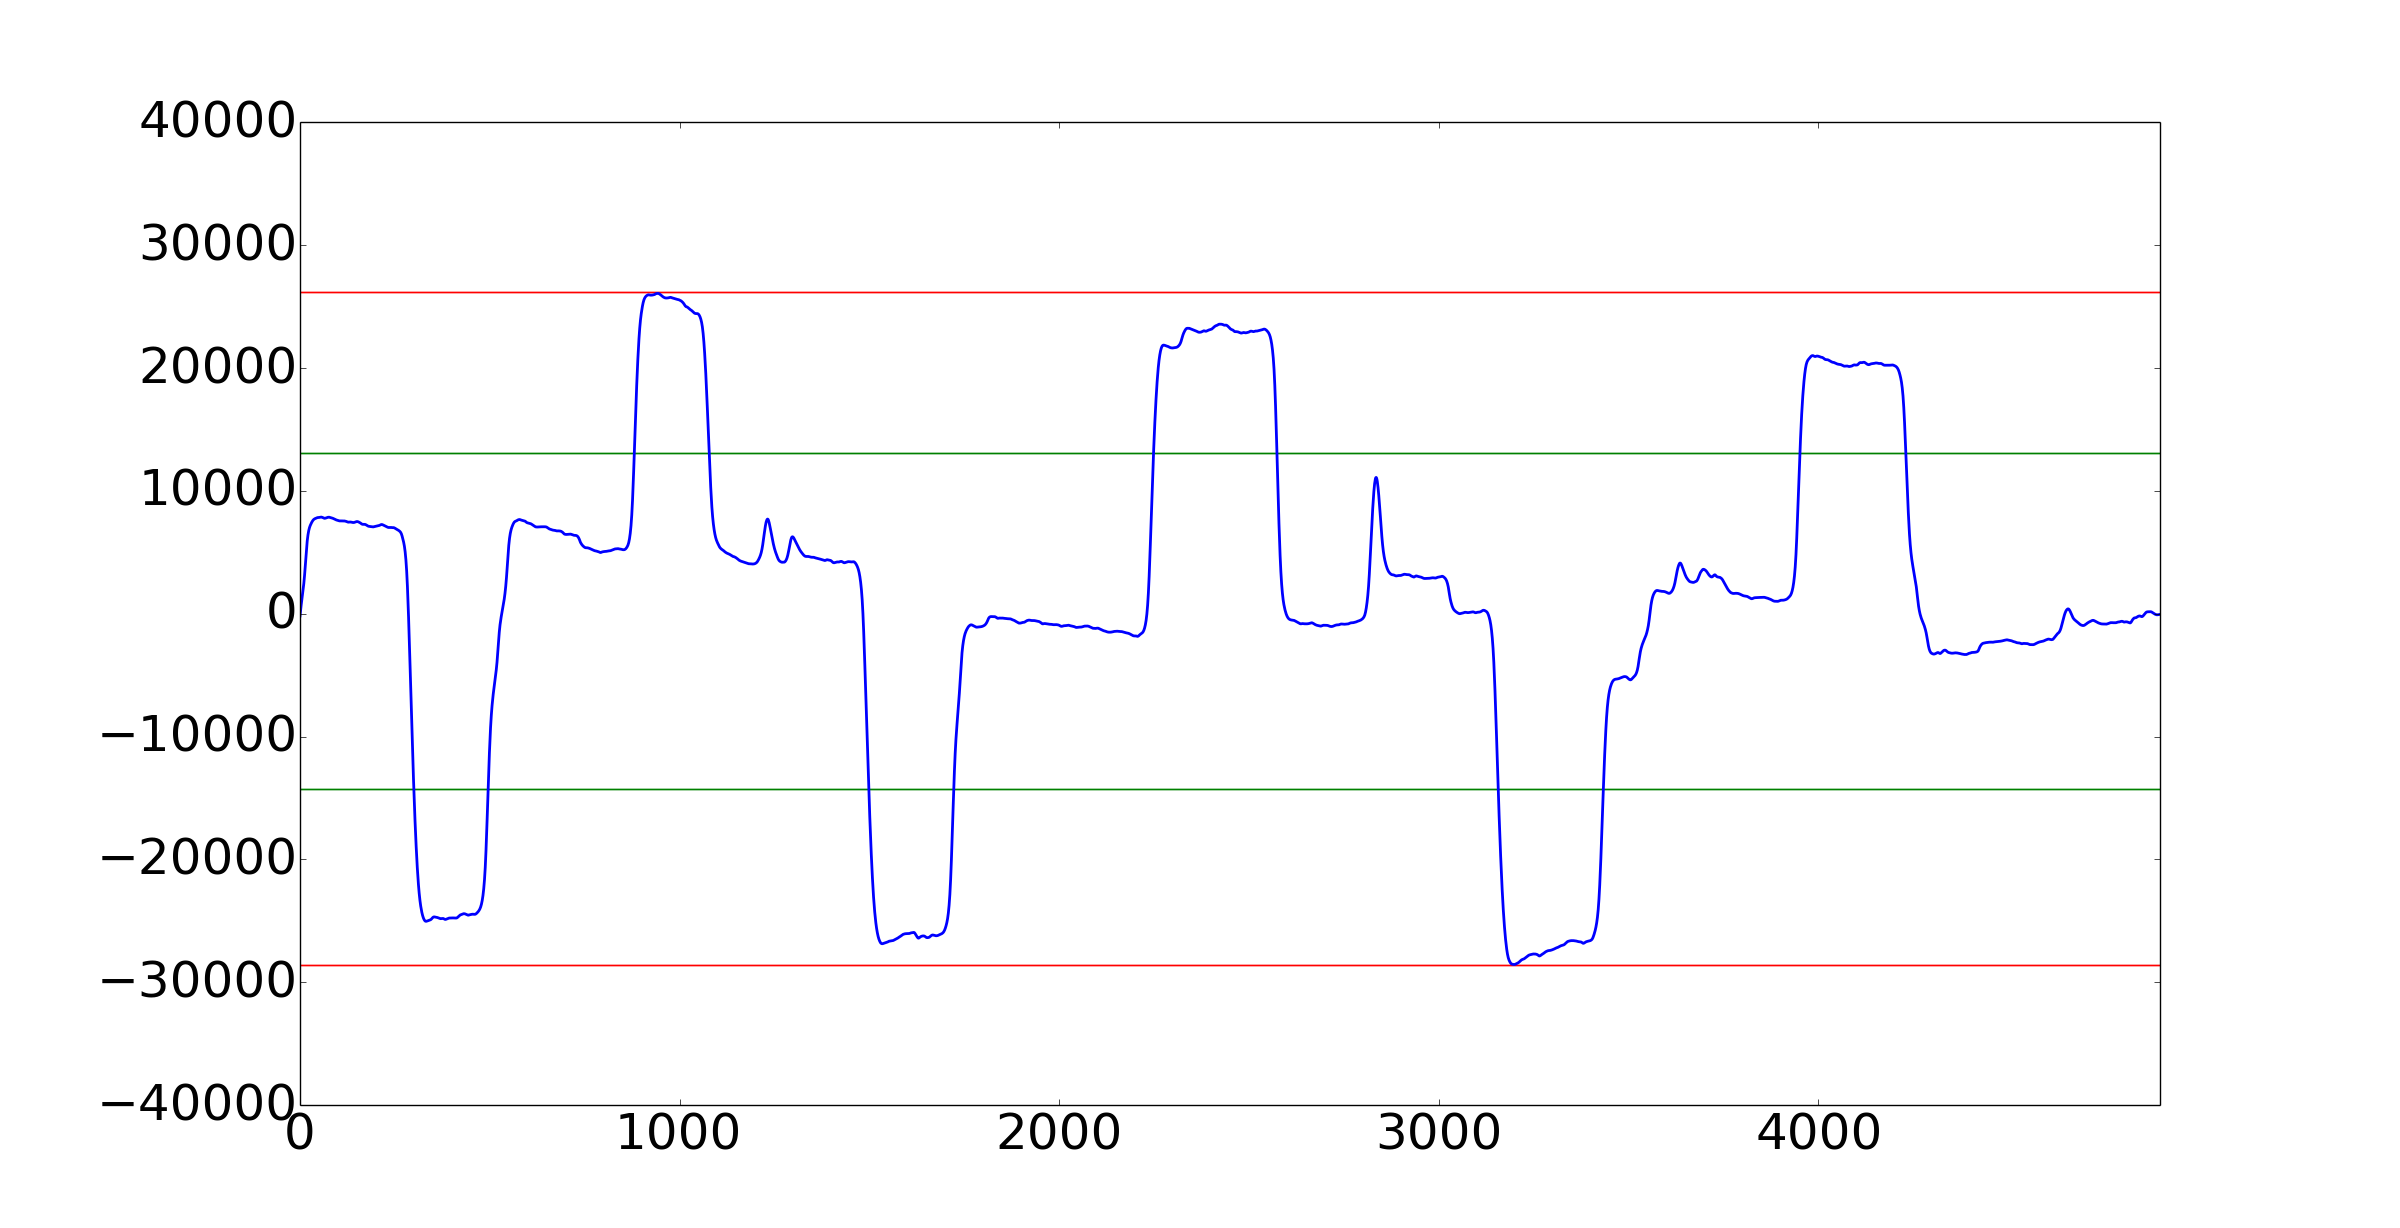
\includegraphics[width=\linewidth]{images/thresholds_distribution}
\caption{In deze afbeelding stellen de rode lijnen het minimum en maximum voor. De groene lijnen zijn het minimum en maximum vermenigvuldigd met $\alpha$.}
\label{fig:maxminthresholds}
\end{figure}

Nu we de bovengrenzen hebben gevonden, moeten we kijkrichtingen gaan zoeken in de nieuwe data. We vragen telkens de 10 recentste datapunten op van de buffer. Om de invloed van een enkele uitschieter in de data te beperken, nemen we telkens het gemiddelde van deze 10 punten. Dit gemiddelde gaan we dan vergelijken met alle bovengrenzen. Slechts wanneer de grenzen 3 opeenvolgende keren overschreden worden, zullen we beslissen dat er een kijkrichting is gevonden.

Omdat we telkens opnieuw de preprocessing-fase uitvoeren op de bufferdata, moeten we oppassen voor het probleem bij veelvuldige herhaling van dezelfde kijkrichting. Zoals eerder vermeld in de thresholds-sectie van gebruikte methoden, zorgt dit voor een verschuiving van het signaal ten opzichte van de y-as. Aangezien we in de herkennings-fase weinig controle hebben over de volgorde van kijkrichtingen, zullen we dit probleem op een andere manier moeten oplossen. Hiervoor gebruiken we afvlakking van het signaal. Telkens als er een threshold overschreden wordt, gaan we het gemiddelde van de vorige 990 datapunten berekenen. Vervolgens vervangen we de originele grensoverschrijdende waardes door dit gemiddelde. Door deze afvlakking, zal de benadering van de biopotentiaal eerder stabiel zijn. Het nadeel van deze techniek is dat de data destructief wordt aangepast en zo mogelijk data verloren gaat. Dit heeft echter geen invloed op dit systeem, aangezien we enkel geïnteresseerd zijn in de nieuwste data. In de figuren~\ref{fig:afvlakking_original} en~\ref{fig:afvlakking} is te zien hoe het signaal veranderd onder afvlakking.

\begin{figure}[h]
\centering
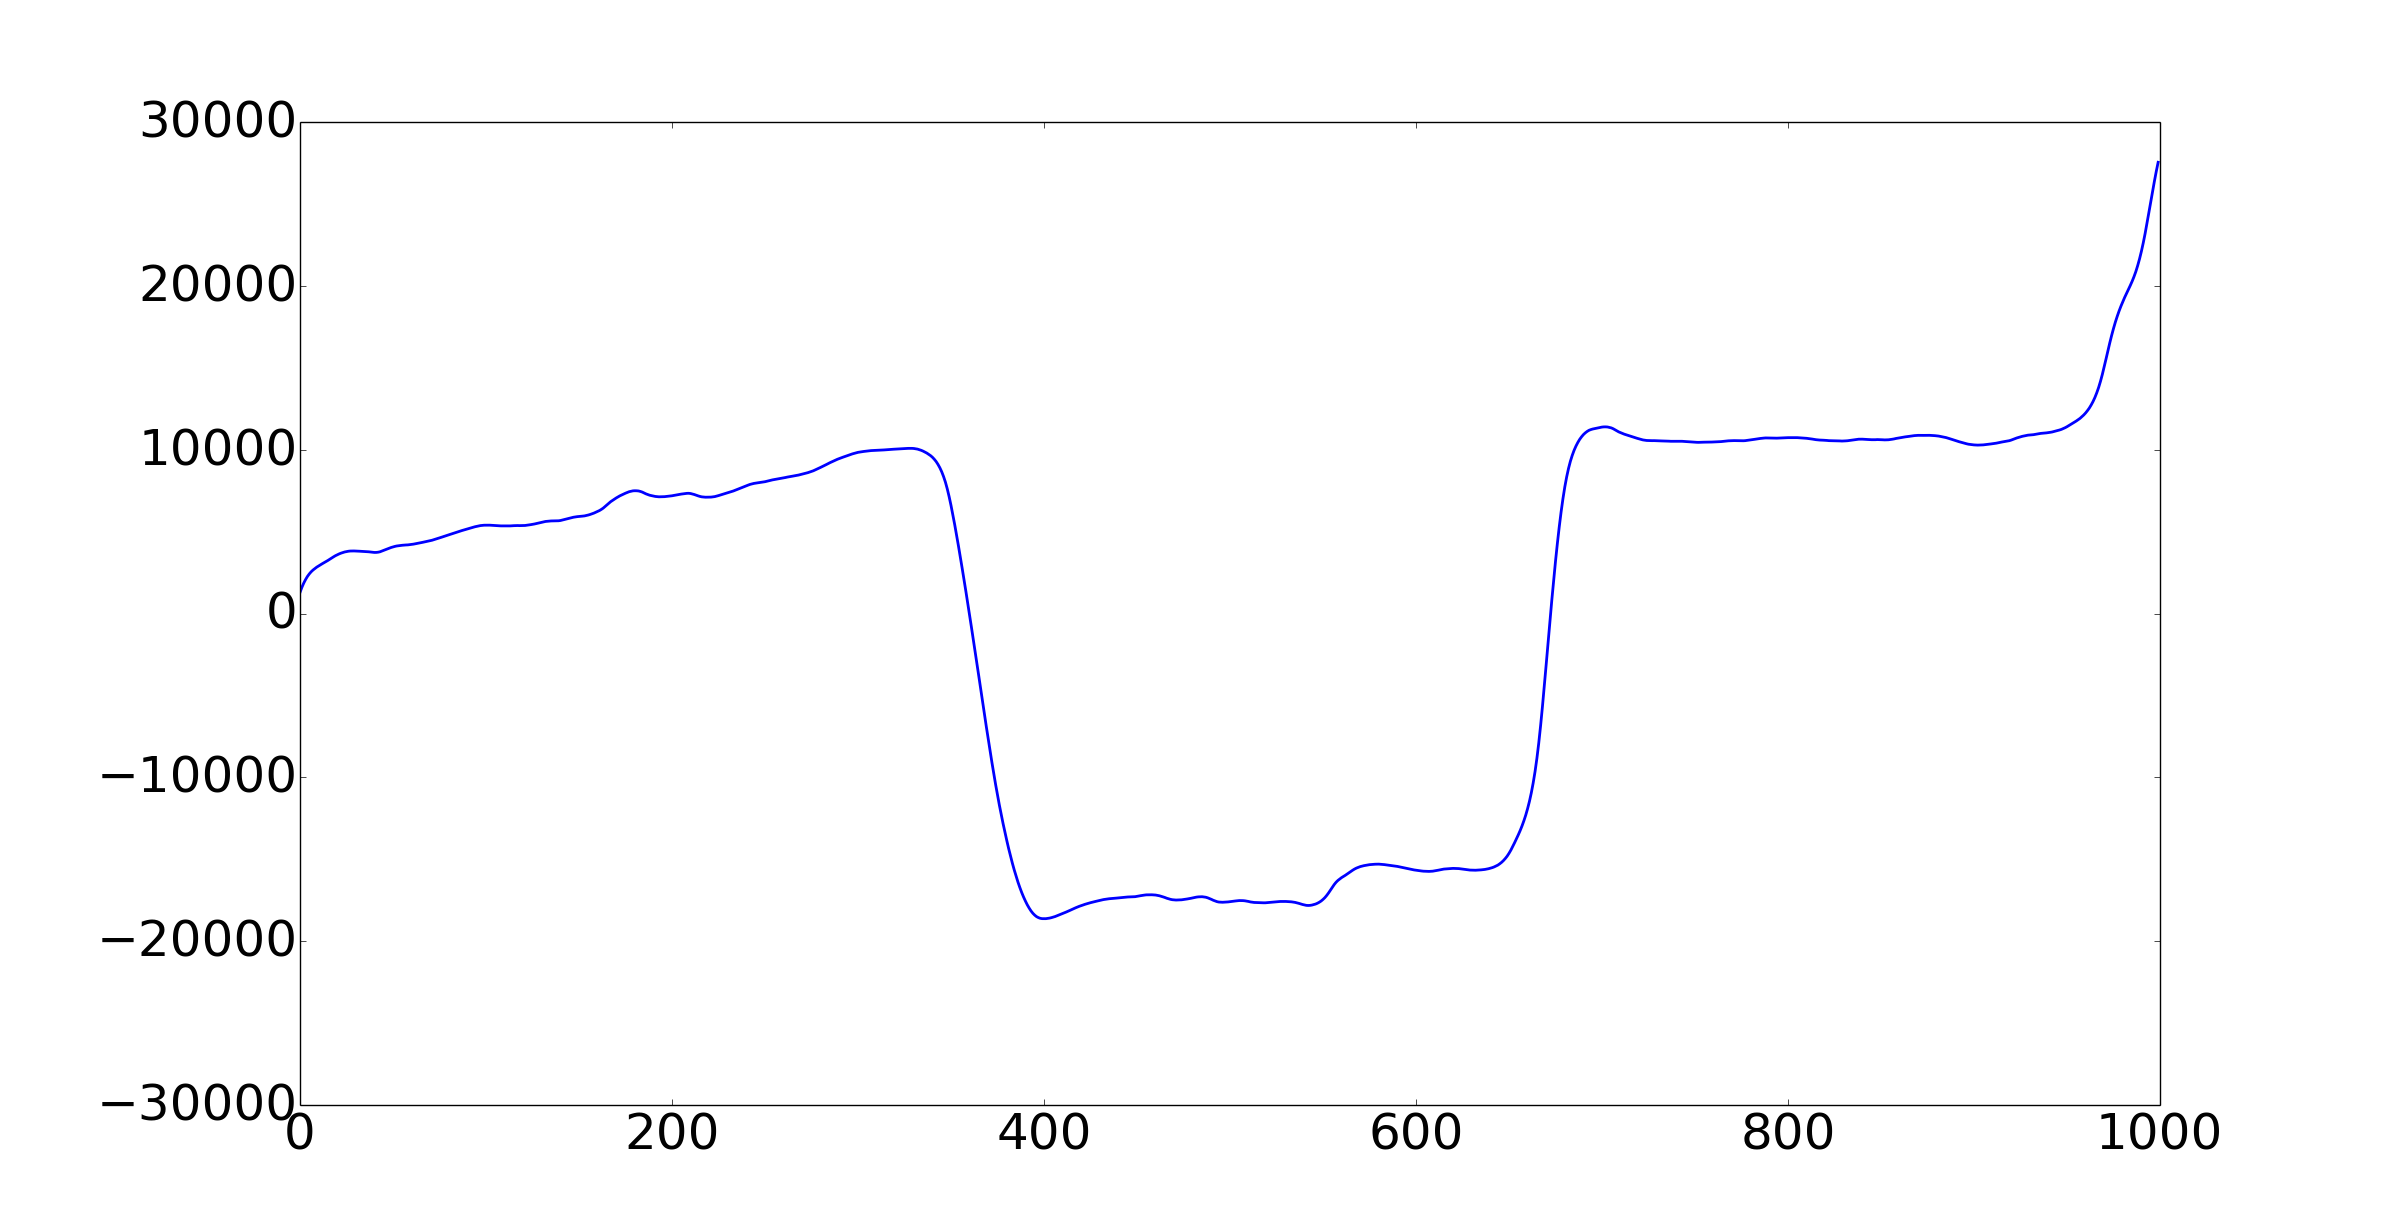
\includegraphics[width=\linewidth]{images/afvlakking_original}
\caption{Dit is een voorbeeld van een gefilterd signaal waarbij geen afvlakking op uitgevoerd is.}
\label{fig:afvlakking_original}
\end{figure}

\begin{figure}[h]
\centering
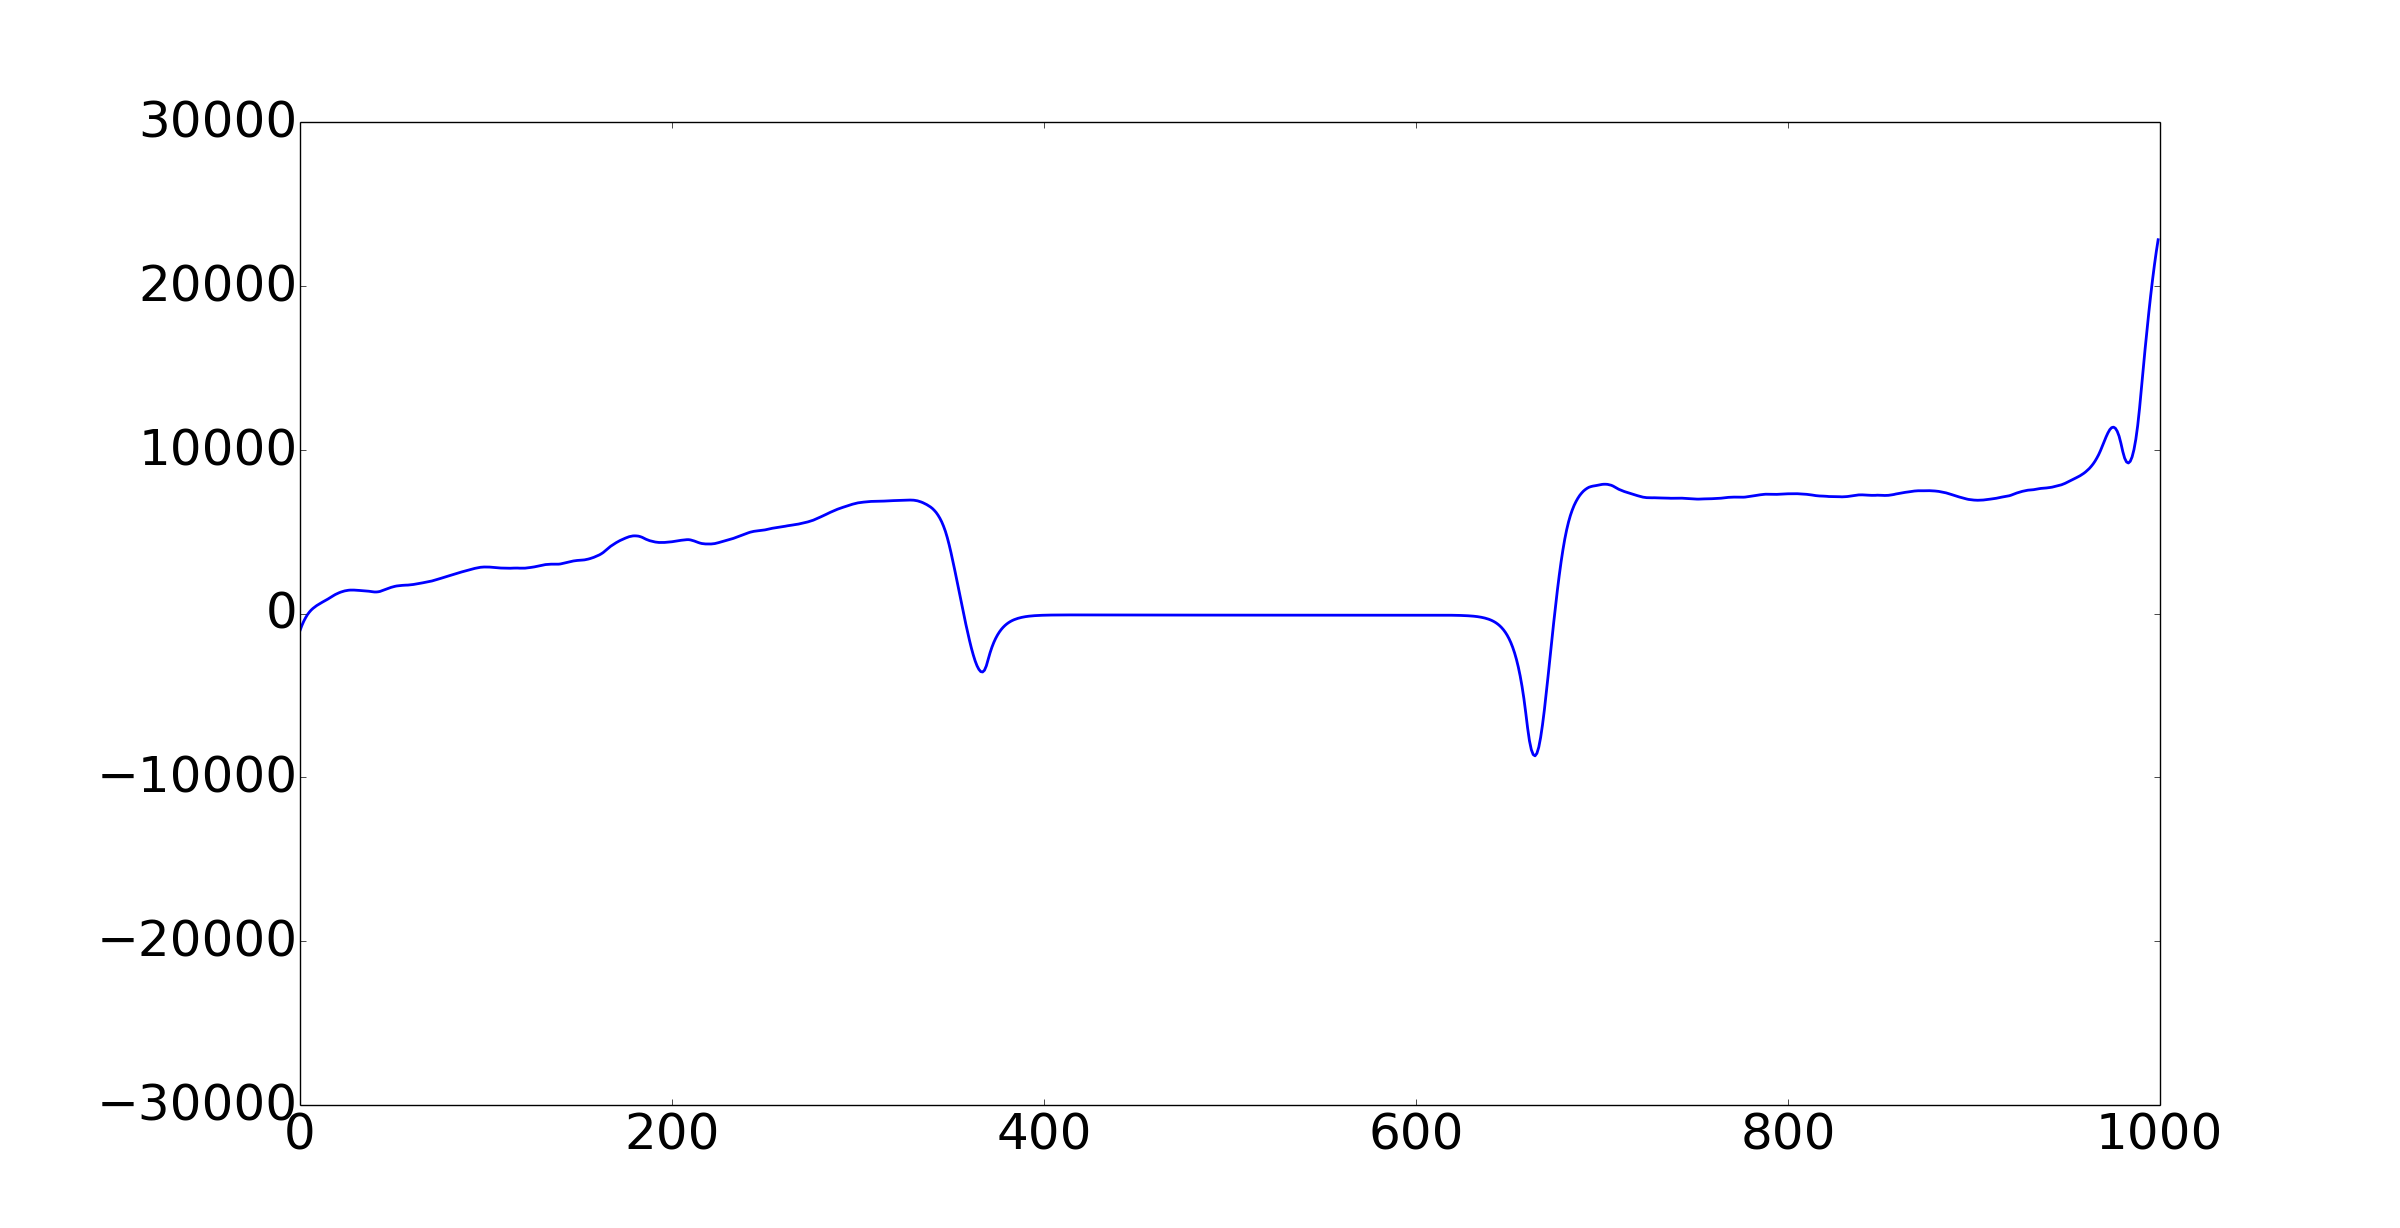
\includegraphics[width=\linewidth]{images/afvlakking}
\caption{Dit is hetzelfde gefilterde signaal uit figuur~\ref{fig:afvlakking_original} waarbij wel een afvlakking op is uitgevoerd. De afvlakking wordt }
\label{fig:afvlakking}
\end{figure}

\subsection{Patronen}

In de calibratie-fase beschikken we over verschillende datasets die gelinkt zijn aan een bepaalde kijkrichting. Voor elke kijkrichting zoeken we minstens één paar van motieven. Deze motieven noemen we het beginmotief en het eindmotief. Een voorbeeld hiervan is te zien in figuur~\ref{fig:beginend}. Deze motieven nemen elk een deel van de hele kijkrichting voor hun rekening. Om telkens zo een paar te verkrijgen, leggen we een aantal voorwaarden op. Zo mogen de motieven elkaar nooit overlappen en moet elk hiervan een verschil in hoogte bestrijken. Dit laatste zorgt ervoor dat we nooit quasi horizontale lijnen, die weinig informatie bevatten, als motief zullen vinden. Wij hebben hiervoor een minimaal verschil van 5000 datapunten gekozen.

\begin{figure}[h]
\centering
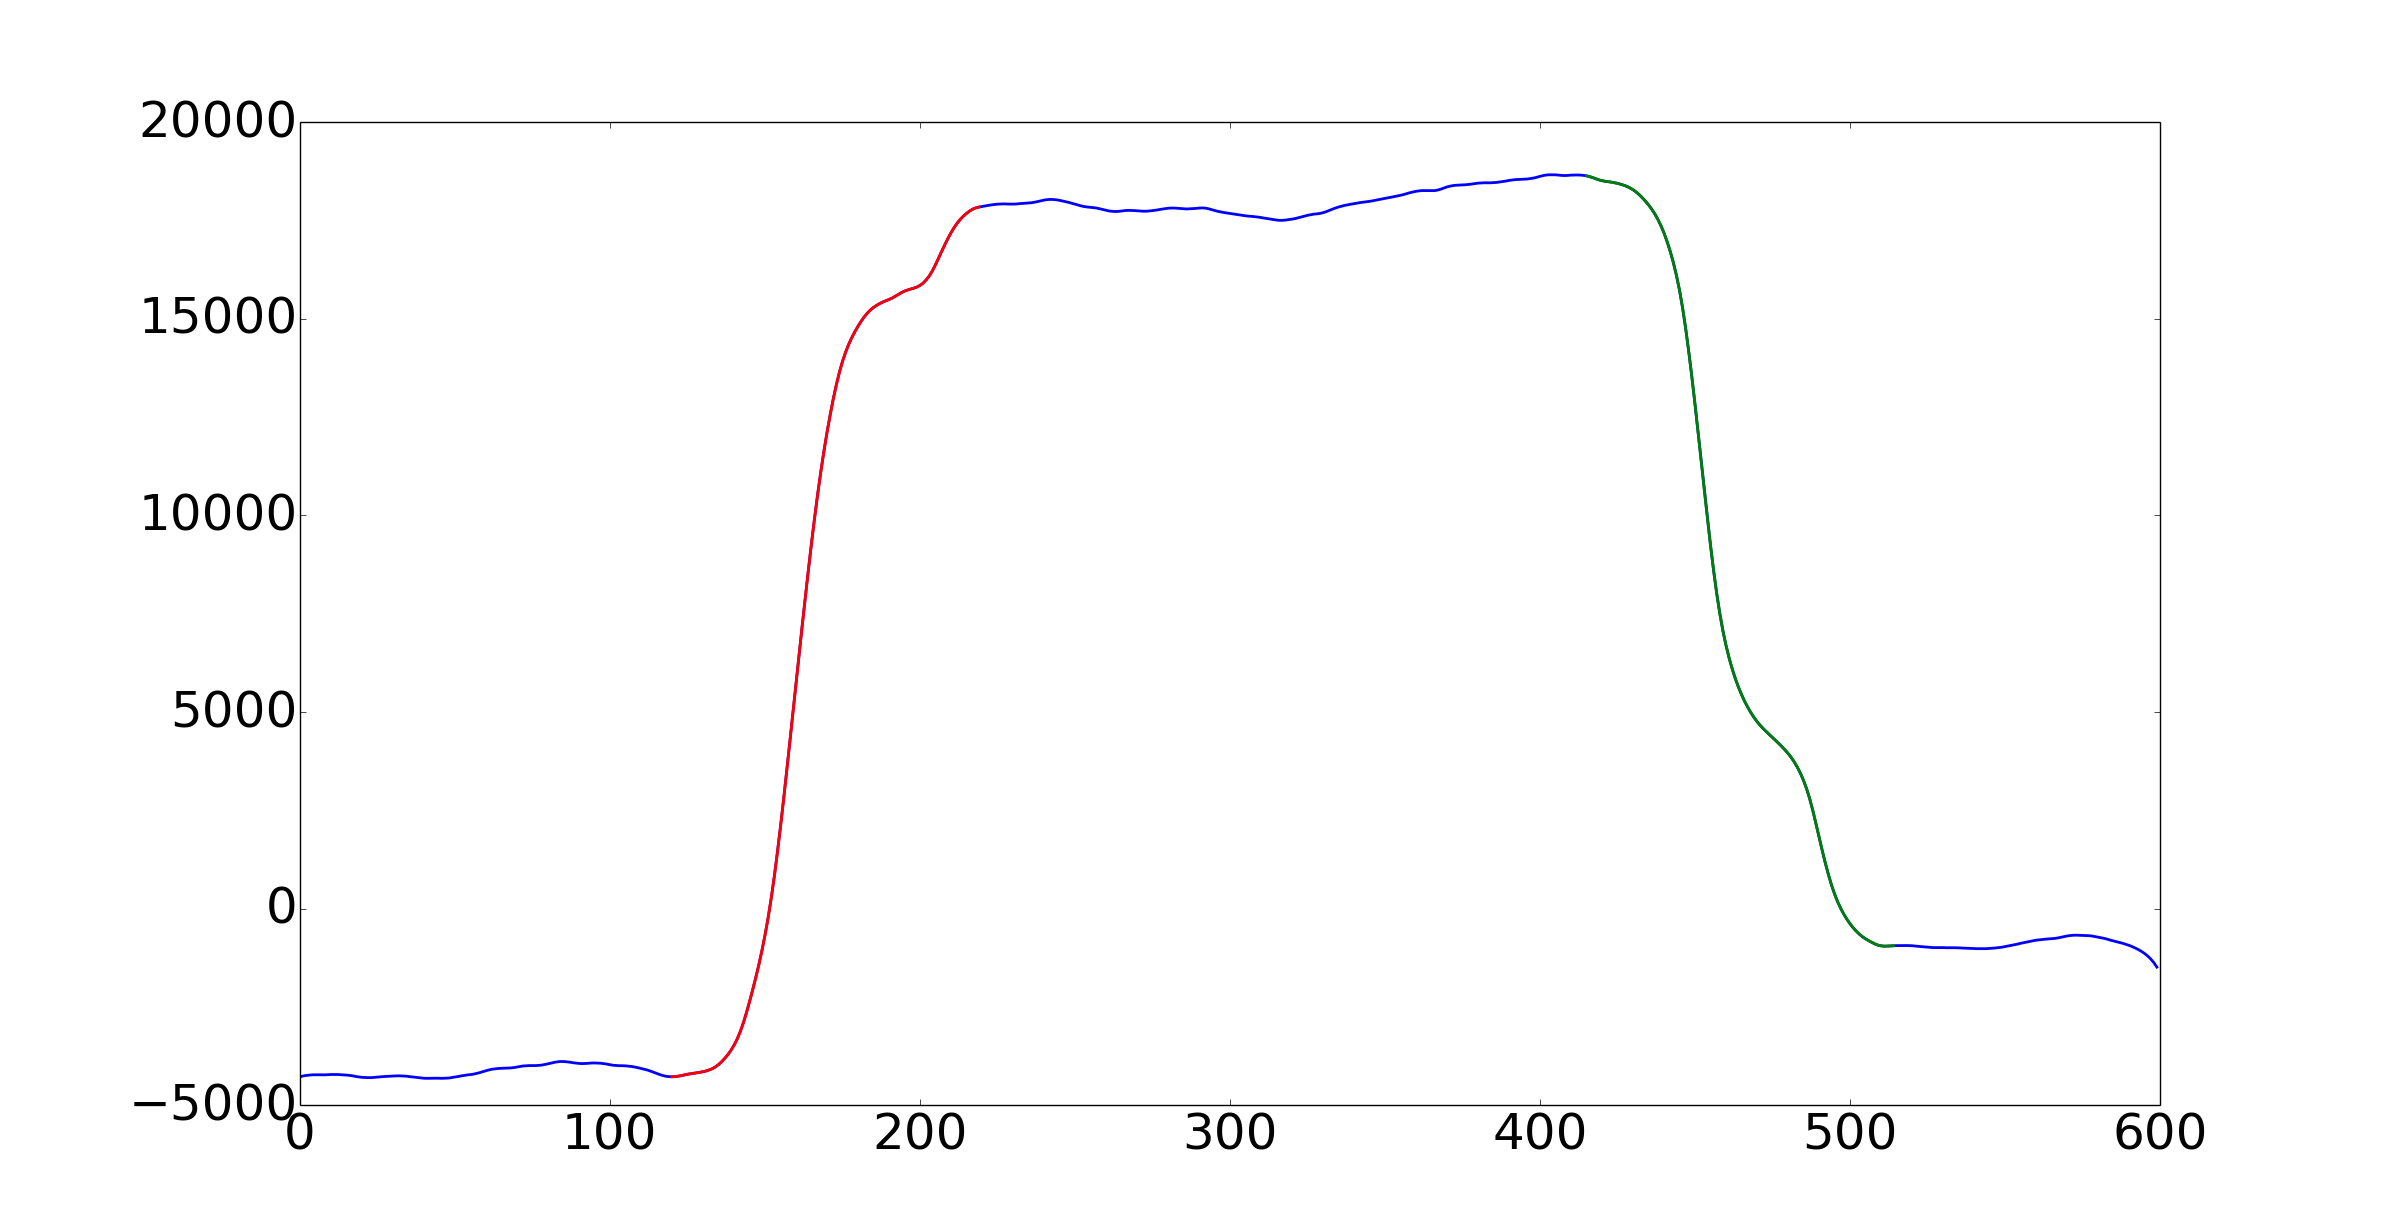
\includegraphics[width=\linewidth]{images/motif_begin_end}
\caption{In deze dataset is het beginmotief aangeduid in het rood en is het eindmotief aangeduid in het groen.}
\label{fig:beginend}
\end{figure}

Voordat we de echte sequenties met elkaar gaan vergelijken, doen we dit eerste met hun genormaliseerde SAX-woorden. Zo kunnen we, zonder al te veel berekeningen, achterhalen welke sequenties in aanmerking komen voor een match. Hiervoor gebruiken we 10 maskers die we op voorhand hebben gedefinieerd. Zo een masker dekt telkens enkele letters van twee te vergelijken SAX-woorden af. Voor elk masker houden we ook een collision matrix bij. Die gebruiken we op de volgende manier. Indien alle overgebleven letters van de SAX-woorden overeen komen, dan wordt de overeenkomstige cel in de collision matrix geincrementeerd. Als we voor alle maskers de collision matrix hebben gemaakt, tellen we al deze matrices met elkaar op. Elk paar van SAX-woorden waarvan de waarde in de overeenkomstige cel van de resulterende matrix groter of gelijk is aan de collision threshold, komt nu in aanmerking voor een match. Deze collision threshold hebben we de waarde 7 gegeven. De oorspronkelijke sequenties van de in aanmerking gekomen SAX-woorden worden nu pas vergeleken. Dit doen we door de euclidische afstand tussen deze genormaliseerde sequenties te berekenen. Pas als deze afstand kleiner is dan de vooraf gedefinieerde range, spreken we van een match.

\begin{table}
\caption{Dit is een voorbeeld van een collision matrix. De letters A tot en met D stellen de verschillende SAX-woorden voor. In dit geval hebben SAX-woorden C en D de meeste collisions, namelijk 10.}
\centering
\begin{tabular}{ l || c | c | c | c }
& A & B & C & D \\ \hline
\hline
A & / & 4 & 2 & 2 \\ \hline
B & / & / & 6 & 3 \\ \hline
C & / & / & / & 10\\ \hline
D & / & / & / & / \\
\hline
\end{tabular}\par
\end{table}

Tijdens de calibratie, vergroten we de collision matrix dynamisch. Dit doen we zodat na de calibratie-fase, niet alle data in één keer verwerkt moet worden, maar wel al tussen door kan gebeuren. Bij de eerste twee sequenties die worden toegevoegd, wordt nog gewoon een collision matrix opgesteld. Bij de derde en volgende sequenties, wordt er een nieuwe rij en kolom toegevoegd die overeenkomt met de nieuwe sequentie. Hiervoor worden de benodigde cellen berekend en ingevuld.

Nu we per sequentie het aantal matches hebben, kunnen we een rangschikking maken. We sorteren alle sequenties op het aantal matches dat ze hebben, met de sequentie met het de meeste matches vooraan. In het geval dat twee sequenties evenveel matches zouden hebben, krijgt de sequentie met de kleinste totale minimale euclidische afstand tot zijn matches voorrang.

In de herkennings-fase worden, na elke nieuwe toevoeging van tien datapunten, de laatste honderd datapunten opgevraagd. Deze worden gezien als een sequentie. Net zoals bij de motieven gebeurde, wordt ook voor deze sequenties gecontroleerd of ze wel een groot genoeg hoogteverschil hebben. De sequentie wordt genormaliseerd en gediscretiseerd naar een SAX-woord. Met behulp van de eerder gebruikte maskers wordt nu ook weer nagegaan of de sequentie goed genoeg lijkt op een motief. Indien de som van alle collisions per masker groter is dan de collision threshold, worden de sequenties zelf weer vergeleken. Indien ze voldoen aan de eerder vermeldde range, wordt het label van het overeenkomstige motief gegeven aan deze sequentie.

Pas wanneer achtereenvolgens het beginmotief en het eindmotief herkend worden, gaan we uit van een kijkrichting. Indien het beginmotief herkend wordt en de herkenning van het eindmotief op zich laat wachten, zal een timer ervoor zorgen dat er niet oneindig lang gewacht wordt op de herkenning van het eindmotief.


\section{Resultaten}
Bij het uitvoeren van experimenten hebben we ons vooral geconcentreerd op the thresholds-methode. Omdat de methode gebruik makend van patronen zoveel afhangt van verschillende parameters, hebben we dit nog niet kunnen optimaliseren.

De opstelling van de experimenten zag er als volgt uit. De sensoren zijn bevestigd op de het gezicht van de gebruiker door middel van stevige plakkers. Deze moeten blijven plakken zonder tussenkomst van de handen. De sensoren die verantwoordelijk zijn voor het meten van de kijkrichtingen links en rechts zijn bevestigd op de slapen, tegen de ooghoeken. [TODO ook zeggen boven en onder?]. De gebruiker zit op een stoel en kijkt voor zich uit. Hierbij is het ook belangrijk dat de gebruiker niet afgeleid kan worden door bewegende voorwerpen. Het gebruiken van andere gezichtsspieren dan de oogspieren moet zo veel mogelijk vermeden worden. De sensoren vangen de signalen van deze spieren namelijk ook op.

We duiden reeksen van kijkrichtingen aan volgens de definitie van reeks~\ref{seq:definitie}. Tijd $t_i$ staat voor het aantal seconden dat ongeveer in de bijhorende kijkrichting gekeken wordt. $h$ geeft aan hoeveel keer de reeks binnen de accolades herhaalt wordt. [TODO beter ding vinden dan \"equation"] [TODO rechtdoor goed?]

\begin{equation}
\label{seq:definitie}
rechtdoor(t_1), \{ links (t_1), rechts (t_2) \} \times h
\end{equation}

In de calibratie-fase werd er telkens volgens reeks~\ref{seq:calibratie} gekeken.

\begin{equation}
\label{seq:calibratie}
\begin{aligned}
&\{rechtdoor(TODO), links(TODO), &\\
&rechtdoor(TODO), rechts(TODO)\} \times 2, &\\
& rechtdoor(TODO)&
\end{aligned}
\end{equation}

Resultaten verwerken we door middel van een confusion matrix. Elke rij en kolom stelt een kijkrichting voor. Op de diagonaal staan alle succesvolle voorspellingen [TODO meer uitleg?]. Aan de hand van deze matrix berekenen we de $accuracy$ (\ref{eq:accuracy}), $recall_k$ (\ref{eq:recall}) en $precision_k$ (\ref{eq:precision}). Hierbij staat $k$ voor de relevante kijkrichting. De kijkrichting $rechtdoor$ geven we een zeer klein gewicht van $1/10$ mee, omdat deze kijkrichting veel gebruikt wordt in de experimenten en een vertekend beeld kan scheppen.

\begin{table}[h]
\caption{Deze tabel stelt de confusion matrix voor.}
\centering
\begin{tabular}{ l || c | c | c }
\backslashbox{Voorspelling~}{Echt~~}
& $links$ & $rechts$ & $rechtdoor$ \\ \hline
\hline
$links$ & a & b & c \\ \hline
$rechts$ & d & e & f \\ \hline
$rechtdoor$ & g & h & i \\
\hline
\end{tabular}\par
\end{table}

[TODO] gewicht van rechtdoor erin verwerken
\begin{equation}
\label{eq:accuracy}
accuracy = \frac{a + e + i}{a + b + c + d + e + f + g + h + i}
\end{equation}

\begin{equation}
\begin{aligned}
\label{eq:recall}
recall_{links} = \frac{a}{a + b + c} \\
recall_{rechts} = \frac{e}{d + e + f}
\end{aligned}
\end{equation}

\begin{equation}
\begin{aligned}
\label{eq:precision}
precision_{links} = \frac{a}{a + d + g} \\
precision_{rechts} = \frac{e}{b + e + h}
\end{aligned}
\end{equation}

\subsection{Experiment 1}

\begin{equation}
\begin{aligned}
\label{seq:exp1}
& \{rechtdoor(TODO), links(TODO)\} \times 5,& \\
& \{rechtdoor(TODO), rechts(TODO)\} \times 5,& \\
& rechtdoor(TODO) &
\end{aligned}
\end{equation}

In dit experiment laten we een gebruiker reeks~\ref{seq:exp1} volgen. Figuur~\ref{fig:experiment1} toont een voorbeeld van hoe het singaal er uitzag.  

\begin{figure}[h]
\centering
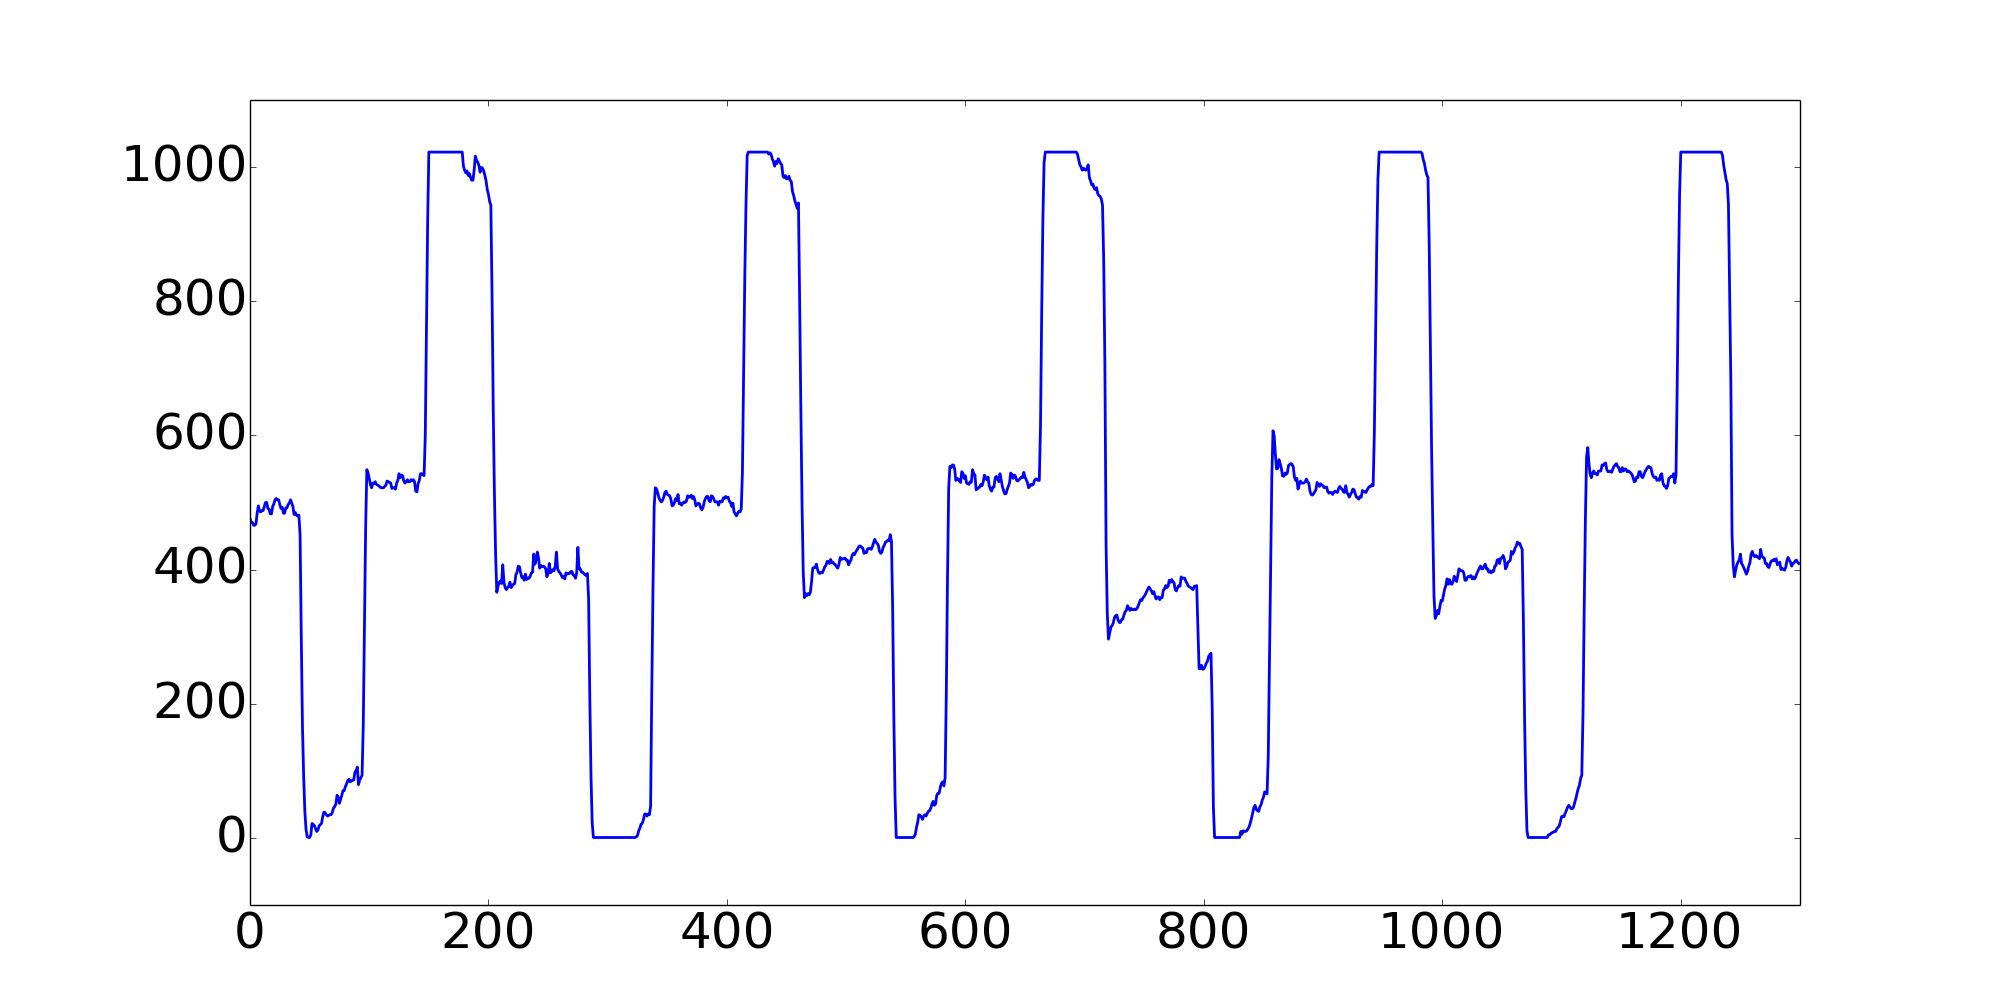
\includegraphics[width=\linewidth]{images/experiment1}
\caption{Een voorbeeld signaal bij uitvoering van experiment 1. [TODO meer uitleg?]}
\label{fig:experiment1}
\end{figure}

\begin{table}[h]
\caption{Confusion matrix na uitvoering van 5 keer reeks~\ref{seq:exp1}.}
\centering
\begin{tabular}{ l || c | c | c }
\backslashbox{Voorspelling~}{Echt~~}
& $links$ & $rechts$ & $rechtdoor$ \\ \hline
\hline
$links$ & a & 0 & 0 \\ \hline
$rechts$ & 0 & e & 0 \\ \hline
$rechtdoor$ & g & h & 55 \\
\hline
\end{tabular}\par
\end{table}

\section{Conclusie}
TODO

\section*{Acknowledgements}
Onder begeleiding van Wannes Meert en prof. Luc De Raedt.
TODO

\appendix

%% The file named.bst is a bibliography style file for BibTeX 0.99c
\bibliographystyle{named}
\bibliography{paper}

\end{document}

